%
\documentclass[12pt]{article}

\usepackage{fullpage}
\usepackage{setspace}
\usepackage{endnotes}
\usepackage{amsmath}
\usepackage{amsfonts}
\usepackage{amssymb}
\usepackage{rotating}
\usepackage{dcolumn}
\usepackage{longtable}
\usepackage{microtype}
\usepackage{graphicx}
\usepackage{url}
\usepackage{natbib}
\bibpunct{(}{)}{;}{a}{}{,}
\usepackage{framed}
\usepackage{lipsum}
\usepackage[font=small,labelfont=sc]{caption}
 \usepackage{float}
\restylefloat{table}
\usepackage[usenames,dvipsnames]{color}

% refs and pdf meta
\usepackage{hyperref}
\hypersetup{
 pdftitle={Reasonable Measures of Uncertainty Under Separation}, % title
 pdfauthor={Carlisle Rainey}, % author
 pdfkeywords={logistic regression}{separation}{Firth}{Cauchy}{MCMC}
 pdfnewwindow=true, % links in new window
 colorlinks=true, % false: boxed links; true: colored links
 linkcolor=BrickRed, % color of internal links
 citecolor=BrickRed, % color of links to bibliography
 filecolor=BrickRed, % color of file links
 urlcolor=BrickRed % color of external links
}

% Set up theorems, etc.
\usepackage{amsthm}
\newtheorem{lemma}{Lemma}
\newtheorem{proposition}{Proposition}
\newtheorem{theorem}{Theorem}
\newtheorem{claim}{Claim}
\newtheorem{assumption}{Assumption}

% Allow restating theorems (for the Appendix)
\usepackage{thmtools}
\usepackage{thm-restate}
\usepackage{cleveref}


% Set up fonts the way I like
\usepackage{tgpagella}
\usepackage[T1]{fontenc}
%\usepackage[T1]{fontenc}
\usepackage[bitstream-charter]{mathdesign}


%Redefine the first level
\renewcommand{\theenumi}{\arabic{enumi}.}
\renewcommand{\labelenumi}{\theenumi}
%Redefine the second level
\renewcommand{\theenumii}{\alph{enumii}.}
\renewcommand{\labelenumii}{\theenumii}
%Redefine the third level
\renewcommand{\theenumiii}{\roman{enumiii}.}
\renewcommand{\labelenumiii}{\theenumiii}
%Redefine the fourth level
\renewcommand{\theenumiv}{\Alph{enumiv}.}
\renewcommand{\labelenumiv}{\theenumiv}


\parskip=0pt
\parindent=20pt
\usepackage{lscape}
\singlespace

% Create footnote command so that my name
% has an asterisk rather than a one.
\long\def\symbolfootnote[#1]#2{\begingroup%
\def\thefootnote{\fnsymbol{footnote}}\footnote[#1]{#2}\endgroup}

\begin{document}


\begin{center}
{\LARGE Reasonable Measures of Uncertainty Under Separation\symbolfootnote[1]{I thank [many people]. Thanks to Mark Bell and Nicholas Miller for making their data available to me. The analyses presented here were conducted with \texttt{R} 3.1.0 and JAGS 3.3.0. All data and computer code necessary for replication are available at \href{https://github.com/carlislerainey/priors.for-separation}{github.com/carlislerainey/priors-for-separation}.}}

\vspace{10mm}

Carlisle Rainey\symbolfootnote[2]{Carlisle Rainey is Assistant Professor of Political Science, University at Buffalo, SUNY, 520 Park Hall, Buffalo, NY 14260 (\href{mailto:rcrainey@buffalo.edu}{rcrainey@buffalo.edu}).}

\end{center}

% remove page number from first page
\thispagestyle{empty}

% abstract
\vspace{10mm}
{\centerline{\textsc{Abstract}}}
\begin{quote}\noindent When facing data sets with small numbers of observations or ``rare events,'' political scientists often encounter important explanatory variables that perfectly predict binary events or non-events. In this situation, maximum likelihood provides implausible estimates and the researcher must incorporate some form of prior information in the estimation. The most sophisticated research uses Jeffreys' invariant prior to stabilize the estimates. While Jeffreys' prior has the advantage of being automatic, I show that, in many cases, it offers too much prior information, providing confidence intervals that are much too narrow. I show that the choice of a more reasonable prior can lead to different substantive conclusions about the likely magnitude of an effect and I offer practice advice for choosing a prior distribution that represents actual prior information.\end{quote}


\newpage
\doublespace

\section*{The Logistic Regression Model}

Political scientists commonly use logistic regression to model the probability of an event of interest. In the typical situation, the researcher uses an $n \times k + 1$ design matrix $X$ consisting of an intercept and $k$ covariates to model a vector $n$ of binary outcomes $y$, where $y_i \in \{0, 1\}$ using the model $\text{Pr}(y_i) = \text{Pr}(y_i = 1 | X) = \dfrac{1}{1 + e^{-X_i\beta}}$, where $\beta$ is a parameter vector of length $k + 1$. 

Using this model, it is straightforward to calculate the likelihood function 

\begin{equation}\nonumber
\text{Pr}(y | \beta) = L(\beta | y) = \displaystyle \prod_{i = 1}^n \left[\left( \dfrac{1}{1 + e^{-X_i\beta}}\right)^{y_i} + \left( \dfrac{1}{1 + e^{-X_i\beta}}\right)^{1 - y_i}\right]\text{.}
\end{equation}

\noindent As usual, one can take the natural logarithm of both sides to calculate the log-likelihood function 

\begin{equation}\nonumber
\log L(\beta | y) = \displaystyle \sum_{i = 1}^n \left[y_i \log \left( \dfrac{1}{1 + e^{-X_i\beta}}\right) + (1 - y_i) \log \left( \dfrac{1}{1 + e^{-X_i\beta}}\right)\right]
\end{equation}

\noindent and take the derivatives of the log-likelihood function to obtain the score function

\begin{equation}\nonumber
\dfrac{\partial \log L(\beta | y)}{\partial \beta} = \displaystyle \sum_{i = 1}^n\left(y_i - \dfrac{1}{1 + e^{-X_i\beta}}\right)X_i\text{.}
\end{equation}

Researchers routinely obtain estimates $\hat{\beta}$ of the model parameters $\beta$ by setting the score function equal to zero and solving for $\beta$ (i.e., maximizing the likelihood of the observed data) and estimate the standard errors are by calculating the square root of the diagonal of the inverse of Fisher's information matrix evaluated at $\hat{\beta}$ (i.e., calculate the curvature around the maximum of the likelihood function to obtain an estimate of the uncertainty of the estimate). While this approach works quite well in most applications, it fails in a situation known as separation \citep{Zorn2005}.

\section*{Separation}

Separation occurs in models of binary outcome data when one explanatory variable (or perhaps a combination of explanatory variables, see \cite{LesaffreAlbert1989}) perfectly predicts zeros, ones, or both. \textit{Complete separation} occurs when the ``problematic'' explanatory variable $s$ (for \textit{s}eparating explanatory variable) perfectly predicts both zeros and ones and \textit{quasicomplete separation} occurs when $s$ perfectly predicts either zeros or ones, but not both (\citealt{AlbertAnderson1984, Zorn2005}). \textit{Overlap}, the ideal case, occurs when no explanatory variable (or combination) perfectly predicts zeros or ones. In this situation, the usual maximum likelihood estimates exist and provide reasonable estimates of parameters. However, under complete or quasicomplete separation, maximum likelihood estimates do not exist (\citealt{AlbertAnderson1984, Zorn2005}).

Complete separation occurs when a covariate perfectly predicts zeros and ones. For example, suppose an explanatory variable $s$ , such that $y = 0$ for $s > 0.5$ and $y = 0$ for $s \leq 0.5$. This corresponds to the middle panel of Figure \ref{fig:illustrating_separation}.  To maximize the likelihood of the observed data, the ``S''-shaped logistic regression curve must assign probabilities of zero when $s \leq 0.5$ and probabilities of one when $s > 0.5$. Since the logistic regression curve lies strictly between zero and one, this likelihood cannot be achieved. However, it can be approached asymptotically as the coefficient for $s$ approaches infinity. Thus, the likelihood function under complete separation is monotonic (has no maximum) and a finite maximum likelihood estimate does not exist.

Quasicomplete separation occurs when a covariate perfectly predicts zeros \textit{or} ones. Figure \ref{fig:illustrating_separation} shows an example pattern in the right panel, where $y$ always equals zero when $s$ equals zero. This situation occurs often in applied political science research with binary inputs. For example, \cite{Gelmanetal2008} find no African-American respondents in their data support Barry Goldwater in 1964, leading to a maximum likelihood estimate of negative infinity for the coefficients for the indicator of African-American respondents. Similarly, \cite{Rauchhaus2009} (see \citealt{BellMiller2014}) finds no instances of states with nuclear weapons engaging in war with each other. In this case, the estimated coefficient for the variable indicating symmetric nuclear dyads (in which both states possess nuclear weapons) equals negative infinity. To maximize the likelihood in this situations, the model must assign probabilities of zero to observations for which $s = 1$ (African-American respondents or symmetric nuclear dyads, in these examples). Again, because the logistic regression curve lies strictly above zero, this cannot happen, though it can be approached asymptotically as the coefficient for $s$ goes to negative infinity. As with complete separation, the likelihood function under quasicomplete separation is monotonic (has no maximum) and a finite maximum likelihood estimate does not exist.

\begin{figure}[H]
\begin{center}
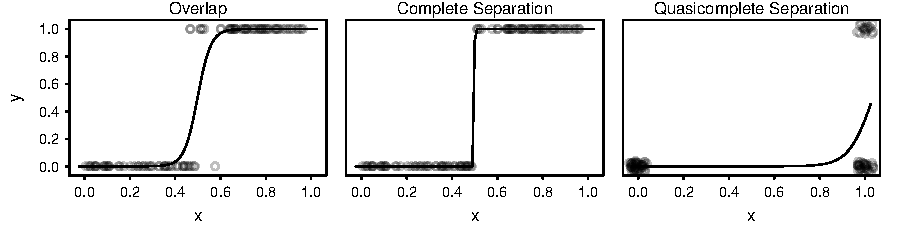
\includegraphics[scale = 1]{figs/illustrate-separation.pdf}
%\vspace{-10mm}
\end{center}
\caption{This figure illustrates overlap, complete separation, and quasicomplete separation as defined by \cite{AlbertAnderson1984}. The maximum likelihood estimates only exist under overlap. Under complete and quasicomplete separation, maximum likelihood fails, returning infinite estimates and standard errors.}\label{fig:illustrating_separation}
\end{figure}

Along coefficient estimates under separation are infinite in theory, the hill-climbing algorithms approximate the infinite estimates with large, finite values that increase with the precision of the algorithm. Table \ref{tab:illustrating_separation} shows the estimates from R's \texttt{glm()} function for each of the hypothetical data sets in Figure \ref{fig:illustrating_separation}. To illustrate the problem, I vary the convergence tolerance between $\epsilon = 10^{-8}$ (the default) and $\epsilon = 10^{-16}$. With the default tolerance, \texttt{glm()} returns very large estimates and standard errors. There is no finite maximum, but the likelihood is flat enough around the large estimates to satisfy the algorithm, given the default tolerance. With the more sensitive tolerance of $\epsilon = 10^{-16}$, the algorithm converges even closer to infinity, but still returns finite estimates. This is a failure of maximum likelihood, because estimates of infinity are usually implausible (i.e., there is always some, though perhaps tiny, probability of a zero or one in any given situation, see \citealt{HeinzeSchemper2002}). 

\begin{table}[H]
\begin{center}
\begin{footnotesize}
\begin{tabular}{l c c | c c | c c }
\hline
 & \multicolumn{2}{c}{Overlap}&\multicolumn{2}{c}{Complete Separation}&\multicolumn{2}{c}{Quasicomplete Separation}\\
               & $\epsilon = 10^{-8}$ & $\epsilon = 10^{-16}$ & $\epsilon = 10^{-8}$ & $\epsilon = 10^{-16}$ & $\epsilon = 10^{-8}$ & $\epsilon = 10^{-16}$ \\
\hline
constant    & $-17.05$ & $-17.05$ & $-739.27$     & $-739.27$     & $-19.57$    & $-26.57$     \\
               & $(5.79)$      & $(5.79)$      & $(139744.58)$ & $(139744.58)$ & $(1520.85)$ & $(50363.70)$ \\
x              & $34.19$  & $34.19$  & $1483.21$     & $1483.21$     & $18.90$     & $25.90$      \\
               & $(11.92)$     & $(11.92)$     & $(280801.40)$ & $(280801.40)$ & $(1520.85)$ & $(50363.70)$ \\
\hline
Log Likelihood & -9.74         & -9.74         & 0.00          & 0.00          & -32.05      & -32.05       \\
Num. obs.      & 100           & 100           & 100           & 100           & 100         & 100          \\
\hline
\multicolumn{7}{l}{Standard errors in parentheses.}
\end{tabular}
\caption{A table providing estimates based on the data shown in Figure \ref{fig:illustrating_separation} using the R function \texttt{glm()} varying the convergence tolerance under overlap, complete separation, and quasicomplete separation. Notice that the estimation algorithm returns estimates and standard errors arbitrarily close to infinity under both types of separation as the tolerances shrinks to zero.}
\label{tab:illustrating_separation}
\end{footnotesize}
\end{center}
\end{table}

Perhaps more starkly, notice  that the strong pattern in the middle panel of Figure \ref{fig:illustrating_separation} does not produce statistically significant result. This is because the likelihood is essentially flat around the ``maximum'' found by the hill-climbing algorithm. As the region around the maximum flattens, the estimates of the standard errors increases. Thus, separation leads to implausible large estimates \textit{and} standard errors. Notice, for example, that while the data in the middle and right panel would almost never occur under the null hypothesis of no relationship, none of the estimates are statistically significant.

\section*{Solutions to Separation}

The maximum likelihood framework (ML) requires the researcher to find the parameter vector that ``maximizes the likelihood of the observed data.'' Of course, infinite coefficients \textit{always} generate separated data, while finite coefficients only generate separation \textit{sometimes}. Thus, under separation, the researcher can only obtain infinite estimates using ML.

Before addressing potential solutions, let me mention two unsatisfactory ``solutions'' found in applied work. In some cases, researchers simply ignore the problem of separation and interpret the large estimates and standard errors as though these are reasonable. However, this approach leads researchers to overstate the magnitude of the effect and the uncertainty of those estimates. A second approach used in practice is to drop the separating variable from the model. \cite{Zorn2005} correctly dismisses this approach:

\begin{quote}
As a practical matter, separation forces the analyst to choose from a number of problematic alternatives for dealing with the problem. The most widely used ``solution'' is simply to omit the offending variable or variables from the analysis. In political science, this is the approach taken in a number of studies in international relations, comparative politics, and American politics. It is also the dominant approach in sociology, economics, and the other social sciences, and it is the recommended method in a few prominent texts in statistics and econometrics. Of course, this alternative is a particularly unattractive one; omitting a covariate that clearly bears a strong relationship to the phenomenon of interest is nothing more than deliberate specification bias.
\end{quote}

As an alternative, \cite{Zorn2005} recommends building prior information $p(\beta)$ into the model using Bayes' rule, so that 

\begin{equation}\nonumber
p(\beta|y) = \dfrac{\overbrace{p(y|\beta)}^{likelihood}\overbrace{p(\beta)}^{prior}}{\int p(y|\beta)p(\beta) d\beta}~\text{.}
\end{equation}

\noindent In this case, the estimate switches to from the maximum likelihood estimate to a summary of the location of the posterior distribution, such as the posterior mode or mean. The current literature on dealing with separation suggests researcher take an automatic approach, adopting Jeffrey's invariant prior distribution.

\subsection*{Jeffrey's Invariant Prior}

\cite{Zorn2005} introduces political scientists to Firth's \citeyear{Firth1993} modified score function (see \citealt{HeinzeSchemper2002} as well). Firth suggests replacing the usual log-likelihood function $\text{log}\,L(\beta | y)$ with a ``penalized'' likelihood function $\text{log}\,L(\beta | y)$, so that $\text{log}\,L^*(\beta | y) = \text{log}\,L(\beta | y)|I(\beta)|^\frac{1}{2}$. It turns out that this penalty is equivalent to Jeffreys' prior for the logistic regression model. The posterior distribution can be obtained by applying Jeffreys' (\citeyear{Jeffreys1946}) rule, which requires setting the prior $p(\beta)$ to be proportional to the square root of the determinant of the information matrix, so that $p(\beta) = |I(\beta)|^\frac{1}{2}$. Then, of course, applying Bayes' rule to obtain the posterior distribution $p(\beta | y) \propto L(\beta | y)|I(\beta)|$, so that Firth's penalty approach is equivalent to a Bayesian approach with Jeffreys' prior.

The usual method of obtaining standard errors is to assume a multivariate normal sampling distribution for the parameter vector $\beta$ and obtain the $(i, j)$ entry of the covariance matrix $\Sigma_\beta$ by calculating the curvature around the maximum likelihood using $\dfrac{\partial^2 \text{log}\,L(\beta | Y)}{\partial \beta_i \partial \beta_j}$ or posterior mode $\dfrac{\partial^2 \text{log}\,\,p(\beta | Y)}{\partial \beta_i \partial \beta_j}$. 

But \citep{HeinzeSchemper2002} and \cite{Zorn2005} point out that this asymptotic approximation of the sampling distribution as normally (symmetrically) distributed might not be appropriate under separation. As an alternative, the suggest using likelihood profiling to obtain the desired confidence interval. They suggest that analysts obtain a $(1 - \alpha)100\%$ confidence interval for the model parameter $\beta_i$ by calculating the (continuous) set of values for which the likelihood-ratio falls below the $(1 - \alpha)100$ percentile of the $\chi^2_1$ distribution \citep{HeinzeSchemper2002}.

However, \cite{Firth1993} did not propose his prior to solve the separation problem. Instead, his purpose was to reduce the well-known small sample bias in logistic regression models. And while it is true that Firth's correction does provide finite estimates under separation, it remains an open question as to whether this automatic prior, designed for other purposes, provides a reasonable estimate of the uncertain of the estimates.

\subsection*{The Cauchy Prior}

Indeed, \cite{Gelmanetal2008} note that Firth's application of Jeffreys' prior is not easily interpretable as an actual application of prior information because the prior $p(\beta) = |I(\beta)|^\frac{1}{2}$. Instead, they suggest an informative prior that, like Jeffreys' prior, bounds the estimates away from positive and negative infinity but has a scale parameter $\sigma$ that allows researchers to choose the amount of prior information provided to the model. They suggest using the Cauchy distribution as priors for the model coefficients.\footnote{Though \cite{Gelmanetal2008} allow for various user-defined prior distributions, they suggest a Cauchy prior centered at zero with scale of 2.5 as a default for appropriately rescaled variables. They suggest rescaling binary inputs to have mean zero and rescaling continuous inputs to have a mean of zero and a standard deviation of one half before estimating the model.}

The Cauchy distribution resembles a normal distribution, but has much heavier tails (it is equivalent to a $t$ distribution with one degree of freedom), which captures the prior belief that the effect is probably smaller, but has some chance of being quite large.

\begin{figure}[H]
\begin{center}
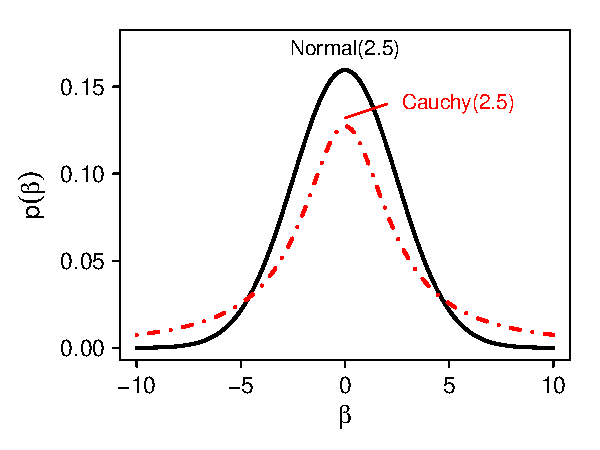
\includegraphics[scale = .8]{figs/illustrate-prior-density.pdf}
\caption{This figure compares the Normal(2.5) and Cauchy(2.5) prior distributions. Notice that the Cauchy distribution has a similar shape to a Normal distribution, but has much heavier tails. Substantively, this prior notes that the coefficient is likely close to zero (e.g. $|\beta| < 2$), but might be quite large (e.g., $|\beta| > 5$).}\label{fig:illustrate-prior-density}
\end{center}
\end{figure}

The posterior distribution is not easily available analytically, but one can easily use MCMC to simulate from the posterior distribution. \footnote{\citep{Gelmanetal2008} obtain standard errors of their estimates by simply calculating the curvature around the posterior mode. They note that although the entire posterior distribution can be computed using MCMC methods, ``it is desirable to have quick calculations that returns a point estimate of the regression coefficients and the standard errors'' (p. 1366). They note that this approximation ``works well in statistical practice and, in addition, recognizes the approximate nature of the model itself.'' However, our purpose is to accurately characterize the uncertainty of the estimates, and asymptotic approximations can underestimate credible intervals by quite a bit.} To facilitate this estimation, I have written an R function, \texttt{cauchy}, to obtain posterior simulations.\footnote{The R package \texttt{MCMCpack} offers some potential to sample from the posterior distribution via a Metropolis-Hastings algorithm with little custom software via the \texttt{MCMClogit()} function. However, the default proposal distribution relies on the large-sample covariance matrix for the parameter estimates. This covariance matrix, of course, is not useful since the variances for the separated variables are much too large. As far as I can tell, the contribution of the large-sample covariance matrix to the proposal distribution is not easily modified. For this reason, I have written custom samplers that use a Metropolis-Hastings algorithm to obtain posterior simulations.} Once a researcher has the MCMC simulations, she can obtain the $(1 - \alpha)100\%$ Bayesian credible interval for parameters by summarizing the simulations.

\section*{The Importance of the Prior}

Choosing a reasonable prior distribution is crucial for dealing with separation in a substantively meaningful manner. In many cases, the data (though the likelihood) swamp the contribution of the prior. However, in the case of separation such that $s_i$ perfectly predicts events, the likelihood determines the shape of the left-hand side of the posterior distribution and the prior (symmetric about zero) determines the shape of the right hand side of the posterior.

The likelihood has an ``S''-shape that approaches a limit of one as the parameter $\beta_s$ for the separating variable $s$ approaches infinity. Thus, for large values of $\beta_s$, the likelihood is essentially flat, which allows the prior distribution to drive the inferences. Thus the prior distribution is not an arbitrary choice made for computational convenience--but a choice that affects the inferences.

\subsection*{The Impact of the Prior in Theory}

Suppose that an explanatory variable $s_i$ perfectly predicts a binary outcome variable $y_i = 1$, such that whenever $s_i = 1$, $y_i = 1$, but when $s_i = 0$, $y_i$ might equal zero or one. \cite{AlbertAnderson1984} refer to this situation as quasicomplete separation. Suppose further an additional set of covariates $X_i$ and the analyst wishes to obtain plausible estimates of coefficients the model $Pr(y_i =1) = \text{logit}^{-1}(\alpha + \beta s_i + X_i \gamma)$. It is easy to find plausible estimates of $\gamma$ using the techniques discussed above (even maximum likelihood usually provides reasonable estimates of these parameters), but finding plausible estimates of $\alpha$ and $\beta$ proves more difficult because maximum likelihood suggests estimates of $-\infty$ and $+\infty$, respectively. In order to obtain a plausible estimate of $\beta$ (which will, in turn, provide a plausible estimate of $\alpha$), the researcher must introduce prior information into the model. My purpose here is to characterize how this prior information impacts the posterior distribution.

In the general situation, the analyst is interested in computing and characterizing the posterior distribution of the coefficient for $s_i$ given the data. Using Bayes' Rule, this posterior depends on the likelihood and the prior, so that $p(\beta | y) = p(y|\beta)p(\beta)$. In particular, the analyst might have in mind a family of priors centered at and monotonically decreasing away from zero with varying scale $\sigma$, so that $p(\beta) = p(\beta|\sigma)$. Suppose that for a particular $\beta^* \geq 0$ the prior distribution is decreasing in $\beta$ at a decreasing rate. Intuitively, this assumption of a $\beta^*$ allows the result to generalize to many common distributions.\footnote{In particular, if the prior distribution is in the form of a double-exponential, which lacks ``shoulders,'' then $\beta^* = 0$. However, the most common prior distributions used in applied work, such as the normal, $t$, and Jeffreys', have ``shoulders'' such that $\beta^* > 0$. In this case, the exact curvature of the distribution in the region $[0, \beta^*]$ affects the relative impact of the prior.} 
Finally, suppose that the informativeness of the prior distribution depends on scale parameter $\sigma$ that is chosen by the researcher and ``flattens'' the prior $p(\beta) = p(\beta | \sigma)$, such that as $\sigma$ increases, the rate a which the prior descends to zero decreases.

\begin{restatable}{theorem}{impact}\label{thm:impact}
The impact of the researchers choice of $\sigma$ on the posterior distribution $p(\beta | y)$ is increasing in $\beta$ for $\beta> \beta^*$. 
\end{restatable}

In many cases, researchers summarize the posterior distribution by providing the 5th and 95th percentiles and a measure of centrality, such as the median.

\begin{quote}
\textsc{Practical Implication of Theorem \ref{thm:impact}:} Under quasicomplete separation where $x_i$ perfectly predicts $y_i = 1$, the prior has a small impact on the lower bound of the 90\% credible interval, a moderate impact on the measures of the location of the posterior (i.e., mean, median, and mode), and a large impact on the upper-bound of the credible interval.
\end{quote}

\subsection*{The Impact of the Prior in Practice}

To illustrate the impact of the prior on inferences when facing separation, I replicate a results from \cite{BarrilleauxRainey2014}, who are interesting in the effect of partisanship on governors' decisions to oppose the Medicaid expansion in their states under the Patient Protection and Affordable Care Act (ACA).\footnote{\cite{BarrilleauxRainey2014} use a logistic regression modeling the probability that a governor opposes the expansion using the following explanatory variables: the partisanship of the governor, the percent of the state's residents who are favorable toward the ACA, whether Republicans control the state legislature, the percent of the state that is uninsured, a measure of the fiscal health of the state, the Medicaid multiplier for the state, the percent of the state that is nonwhite, and the percent of the state that resides in a metropolitan area. See their paper for more details.} As the authors note, no Democrats opposed the expansion leading to a problem of separation. I use MCMC to simulate from the posterior using several different prior distributions, including Jeffreys' prior \citep{Zorn2005} and the Cauchy prior with scales of 1, 2.5, and 5 \citep{Gelmanetal2008}. While the choice of prior does not affect the conclusion about the \emph{direction} of the effect, it has a large impact on the conclusion about the \emph{magnitude} of the effect. This can be especially important when researchers are making claims about the substantive importance of their estimated effects (see \citealt{Rainey2014}, \citealt{Gross2014}, and \citealt{McCaskeyRainey2014}).

Figure \ref{fig:matters-post} shows the posterior distribution for the coefficient for the indicator of Republican governors. Notice that the different priors lead to different posterior distributions. Notice, in particular, that the choice of the prior has a large impact on the right-hand side of the posterior. More informative priors (e.g., Jeffrey's prior) lead to a more peaked posterior distribution that rules out very large effects. Less informative priors (e.g., Cauchy(2.5)) lead to the conclusion that even large effects are plausible. These differences affect the conclusions that the researchers draw about the likely magnitude of the effect.

\begin{figure}[H]
\begin{center}
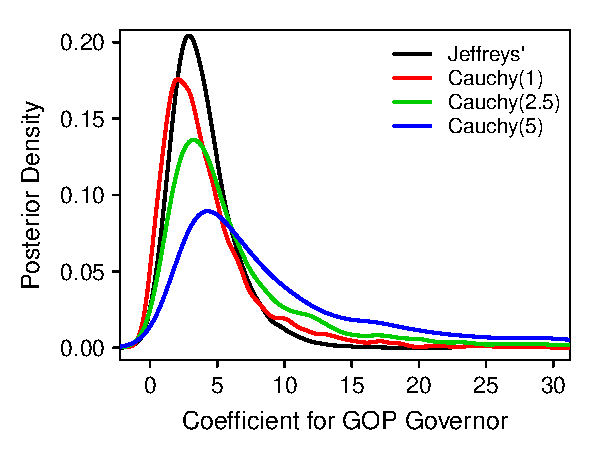
\includegraphics[scale = .8]{figs/matters-post.pdf}
\caption{This figure provides the posterior distribution for the coefficient of the indicator for GOP governors in the model offered by \cite{BarrilleauxRainey2014}. Notice that the location and the spread of the posterior depend on the prior chosen, especially the right-hand side of the distribution.}\label{fig:matters-post}
\end{center}
\end{figure}

Figure \ref{fig:matters-ci} shows how the choice of prior impacts the 90\% credible interval. Notice that different prior distributions lead to different conclusions about the plausible values of the effect. In particular, different priors lead to different conclusions about the upper-bound on the plausible effect sizes. For example, Jeffreys' prior, the default proposed by \cite{Zorn2005} and \cite{HeinzeSchemper2002}, suggests the effect lies in the range $\beta_{\text{GOP Gov.}} \in [0.9, 8.4]$, with a posterior mean of 3.9. On the other hand, the less informative Cauchy(2.5) prior, the default proposed by \cite{Gelmanetal2008}, suggests the effect lies in the range $\beta_{\text{GOP Gov.}} \in [1.0, 22.5]$, with a posterior mean of 7.3. A simple change from one proposed default to another more than doubles the upper bound on the 90\% credible interval and almost doubles the posterior mean. Further, the Cauchy(5) prior, a plausible prior if one believes the effect might be large, produces the upper-bound on the 90\% credible interval from is more than four times larger than the upper-bound produced by Jeffrey's prior. The posterior mean from the Cauchy(5) prior is larger falls above the upper-bound from the 90\% credible interval from Jeffrey's prior.

\begin{figure}[H]
\begin{center}
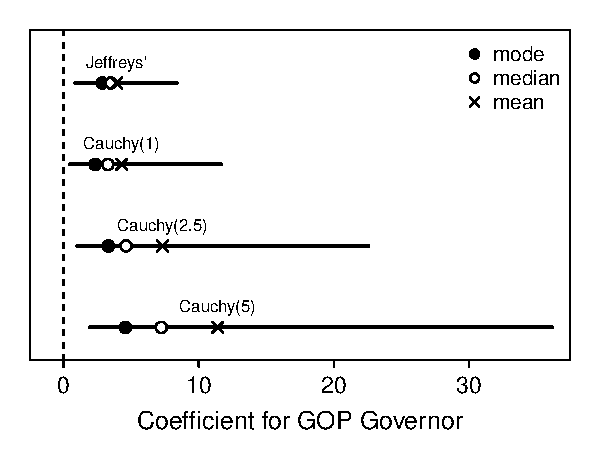
\includegraphics[scale = .8]{figs/matters-ci.pdf}
\caption{This figure provides the (equal-tailed) 90\% credible intervals for the coefficient of the indicator for GOP governors in the model offered by \cite{BarrilleauxRainey2014}. Notice that the location and the spread of the posterior depend on the prior chosen, especially the right-hand side of the distribution. Note that Jeffrey's prior, suggested by \cite{Zorn2005}, is the most informative of these priors, suggesting that a coefficient smaller than about 10 is quite unlikely. On the other hand, credible interval using the Cauchy(2.5) prior, as suggested by \cite{Gelmanetal2008}, is about \emph{twice} as wide as the credible interval from Jeffreys' prior. Finally, notice that the Cauchy(5) prior--a plausible prior if the researcher believes the effect might be large--produces a posterior mean larger than the upper bound of the 90\% credible interval using Jeffrey's prior.}\label{fig:matters-ci}
\end{center}
\end{figure}

This leads us to conclude that the choice of prior matters--it affects the inferences that we draw from the data. It is not sufficient to rely on the prior distribution designed as a default for other purposes. Instead, we must rely on prior distributions that represent actual prior information about the likely magnitude of the coefficients.



\clearpage
\bibliographystyle{apsr_fs}
\bibliography{/Users/carlislerainey/Dropbox/papers/bibliography/bibliography.bib}

\clearpage
\begin{appendix}
\begin{center}
\LARGE{\textbf{Online Appendix}}\vspace{4mm}
\end{center}

\section*{Proof of Theorem \ref{thm:impact}}

\begin{assumption}[Separation]
Suppose quasicomplete separation such that $s_i$ perfectly predicts $y_i = 1$. 
\end{assumption}

\begin{assumption}[Prior Shape]
Suppose that the researcher computes the posterior distribution $p(\beta | y) = p(y | \beta)p(\beta)$ such that for a particular $\beta^* \geq 0$ the prior distribution is decreasing at a decreasing rate.
\end{assumption}

Intuitively, this assumption of a $\beta^*$ allows the result to generalize to a range of common distributions. In particular, if the prior distribution is in the form of a double-exponential, which lacks ``shoulders,'' then $\beta^* = 0$. However, the most common prior distributions used in applied work, such as the normal, $t$, and Jeffreys', have ``shoulders'' such that $\beta^* > 0$. In this case, the exact curvature of the distribution in the region $[0, \beta^*]$ affects the relative impact of the prior.

\begin{assumption}[Scale Parameter]
Suppose finally the that informativeness of the prior distribution depends on scale parameter $\sigma$ ``flattens'' the prior $p(\beta) = p(\beta | \sigma)$, such that as $\sigma$ increases, the rate a which the prior descends to zero decreases.
\end{assumption}

$\sigma$ is chosen by the researcher based on prior information about the likely values of the coefficients.

Before proving Theorem \ref{thm:impact}, it is helpful to show several initial results.

\begin{lemma}\label{thm:L1}
$\dfrac{\partial p(y | \beta)}{\partial \beta} > 0$ for all $\beta$. 
\end{lemma}

\begin{proof}[Proof of Lemma \ref{thm:L1}]
The quantity $p(y | \beta)$ is the probability of observing $y$ (i.e., an outcome variable separated by $s$). Increasing values of $\beta$ make this separation increasingly likely. Thus, $p(y | \beta)$ is increasing in $\beta$ so that $\dfrac{\partial p(y | \beta)}{\partial \beta} > 0$. 
\end{proof}

\begin{lemma}\label{thm:L2}
$p(\beta | \sigma) > 0$ for all $\beta$.
\end{lemma}

\begin{proof}[Proof of Lemma \ref{thm:L2}]
The quantity $p(\beta | \sigma)$ is a probability distribution defined to have support over the real line and thus $p(\beta | \sigma) > 0$ for all $\beta$. 
\end{proof}

\begin{lemma}\label{thm:L3}
$p(y | \beta) > 0$ for all $\beta$.
\end{lemma}

\begin{proof}[Proof of Lemma \ref{thm:L3}]
The quantity $p(y | \beta)$ is a probability and thus bounded between zero and one. As long as data lie within the support of the probability model, this quantity lies strictly above zero. Since the theorem defines the data as such, $p(y | \beta) > 0$.
\end{proof}

\begin{lemma}\label{thm:L4}
$\dfrac{\partial^2 p(\beta | \sigma)}{\partial \beta \partial \sigma}$ for $\beta > \beta^*$.
\end{lemma}

\begin{proof}[Proof of Lemma \ref{thm:L4}]
By assumption, the prior density is decreasing at a decreasing rate in $\beta$ for all $\beta > \beta^*$. Also by assumption, the scale parameter $\sigma$ controls the rate at which $\beta$ decreases such that increasing $\sigma$ leads to a slower rate of decrease. These two assumptions together imply that $\dfrac{\partial^2 p(\beta | \sigma)}{\partial \beta \partial \sigma}$ for $\beta > \beta^*$.
\end{proof}

Now recall Theorem \ref{thm:impact}:

\impact*

\begin{proof}[Proof of Theorem \ref{thm:impact}]
To show that the effect of $\sigma$ is increasing in $\beta$, I simply need to show that $\dfrac{\partial^2 p(\beta | y)}{\partial \beta \partial \sigma} > 0$ for $\beta > \beta^*$. 

Recall that the posterior $p(\beta | y)$ is proportional to the likelihood $p(y | \beta)$ times the prior $\beta(\beta | \sigma)$, so that $p(\beta | y) \propto p(y|\beta)p(\beta | \sigma)$. First, we can use the product rule to obtain the derivative of $p(\beta | y)$ so that 

\begin{equation}\nonumber
\dfrac{\partial p(\beta | y)}{\partial \beta} \propto \dfrac{\partial p(y | \beta)}{\partial \beta} p(\beta | \sigma) + p(y | \beta)\dfrac{\partial p(\beta | \sigma)}{\partial \beta \partial}\text{}.
\end{equation}

\noindent Only the final term involves $\sigma$, so we can easily obtain the desired derivative

\begin{equation}\label{eqn:cross-partial}
\dfrac{\partial^2 p(\beta | y)}{\partial \beta \partial \sigma} \propto \overbrace{\dfrac{\partial p(y | \beta)}{\partial \beta}}^{\text{Lemma 1}:~+} \overbrace{p(\beta | \sigma)}^{\text{Lemma 2}:~+} + \overbrace{p(y | \beta)}^{\text{Lemma 3}:~+} \overbrace{\dfrac{\partial^2 p(\beta | \sigma)}{\partial \beta \partial \sigma}}^{\text{Lemma 4}:~+}\text{.}
\end{equation}

\noindent Each term on the right-hand side of Equation \ref{eqn:cross-partial} is positive  for $\beta > \beta^*$ (Lemmas 1-4), so that $\dfrac{\partial^2 p(\beta | y)}{\partial \beta \partial \sigma} > 0$ for $\beta > \beta^*$.

\end{proof}

\end{appendix}
\end{document}



